\documentclass[review]{elsarticle}

\usepackage[]{geometry}
\usepackage{amsmath}
\usepackage{amssymb}
\usepackage{tikz}
\usepackage{graphicx}
\usepackage{hyperref}
\usepackage{natbib}
\bibliographystyle{elsarticle-harv}
\biboptions{authoryear}

\newcommand{\ra}{\rightarrow}
\newcommand{\afs}[2]{\Phi_{#1}^{(#2)}}
\newcommand{\Dfrac}[2]{%
  \ooalign{%
    $\genfrac{}{}{1.2pt}0{#1}{#2}$\cr%
    $\color{white}\genfrac{}{}{.4pt}0{\phantom{#1}}{\phantom{#2}}$}%
}
\newcommand{\cond}{\middle\vert}

\newcommand{\sgcomment}[1]{\textcolor{red}{SG: #1}}
\newcommand{\ikcomment}[1]{\textcolor{blue}{IK: #1}}

\journal{Theoretical Population Biology}

\begin{document}
\begin{frontmatter}
  \title{Models of strong selection in large samples}

  \author{Ivan Krukov}
  \author{Simon Gravel}

  \begin{abstract}
    
    Neutral models of genetic diversity tend to be easier to analyze than models including
    selection. Under the neutral Wright-Fisher model, the number of lineages that contribute to
    ancestry of a sample decreases back in time due to coalescent events. As a consequence, useful
    recursion equations can be derived for patterns of polymorphism. By contrast, under negative
    selection, the number of relevant lineages can increase as we go back in time, due to selective
    deaths. As a result, the equivalent recursi`on equations do not close. However, given a
    sufficiently large sample size, the expected reduction in the number of contributing lineages
    due to coalescence is larger than the increase due to selection, so the net number is unlikely
    to increase. We use this observation to derive asymptotically closed recursion equations for the
    distribution of allele frequencies in finite samples. We show that this approach is accurate
    under strong drift and strong natural selection. We derive several asymptotic results to
    determine when the sample size is sufficiently large for drift to overcome the effect of
    selection.
  \end{abstract}

\end{frontmatter}

\section{Introduction}
\label{sec:introduciton}

The allele frequency spectrum (\textit{AFS}) is an important summary of genetic diversity that is
commonly used to infer demographic history and natural selection \citep{}. Given a demographic
scenario of population size histories and migrations, the diffusion approximation or coalescent
simulations can be used to obtain a predicted \textit{AFS} \citep{}. By comparing
predictions to the observed \textit{AFS}, one can compute likelihoods for different demographic
scenarios. Unfortunately, the \textit{AFS} calculations can be time consuming with complex
demographic models, for example with multiple populations, or with large sample sizes \citep{}.

In the absence of selection, efficient computational shortcuts can be used. In particular, recursion
equations have been derived for moments of the allele frequency distribution
\citep{KimuraCrow1964,Ewens1972,JouganousEtAl2017}. Recently, these recursions have been useful in
fitting complex demographic models to genetic data \citep{JouganousEtAl2017,KammEtAl2017}.
 
In the presence of natural selection, the corresponding recursion equations do not close
\citep{Donnelly, JouganousEtAl2017} -- they form an infinite set of coupled ordinary differential
equations. Moment-based closure approximation have been developed \citep{JouganousEtAl2017}, but
these are not robust to strong selection and their convergence properties are not well understood.

Closure of the moment equations under the neutral Wright-Fisher model occurs because the number of
parental lineages that contribute to the present day sample is equal to or smaller than the sample
size, due to coalescent events back in time \citep{Kingman1982a}. To describe a sample of size $n$,
we need to recursively consider samples of size $n'\le n$. This does not hold under negative
selection -- due to selective deaths, the number of parental lineages $n'$ can be larger than $n$.
As we demonstrate later, this leads to a potentially infinite number of terms in the equations. This
is similar to the ancestral selection graphs (\textit{ASG}), \citep{KroneNeuhauser1997}, where the
number of relevant lineages can increase back in time.

The interplay of drift and selection is important to consider. In large sample sizes, there are many
more common ancestry events than selective deaths, so the number of contributing lineages is
unlikely to increase back in time. This suggests that large sample sizes can lead to
almost-closed recursion equations, as we will demonstrate here.

An additional complication is multiple and/or simultaneous coalescent events -- which emerge with
large sample sizes \citep{BhaskarEtAl2014}. The standard coalescent model only allows one event per
generation, but we also need to consider higher-order events, \textit{e.g.} multiple two-lineage or
three-lineage mergers. These multiple-lineage coalescent events oppose the effect of selection by
rapidly decreasing the number of contributing lineages \citep{NelsonEtAl2019}.

In this article we derive these asymptotically-closed recursions in the Wright-Fisher model, and
study their behavior and applications for modeling the distribution of allele frequencies under
strong selection.

%Unlike the \textit{ASG}, the present method does not need to assume an infinitely large population
%size, and also explicitly tracks multiple coalescent events, which is important with large sample
%sizes \citep{BhaskarEtAl2014}. Our approach can also be combined with the jackknife. Unlike the
%jackknife, our method allows derivation of bounds on the performance of the approximation.

\section{Background}
\label{sec:background}

We consider a haploid Wright-Fisher model of size $N$, focusing on a single biallelic locus. For a
present sample with $n_o$ offspring lineages at time $t$, we will be looking for recursion equations
for the allele frequency distribution by considering the sampling process for a finite sample under drift 
and selection.   

To model selection, we imagine that all parents generate 
a large number of gametes, and that offspring pick gametes at random. Draws from the deleterious allele are 
rejected with probability $s$, triggering a re-draw (Fig.\ref{fig:schematic}B). This leads to a $1:1-s$ advantage 
in favour of the advantageous allele, and makes explicit the number of lineages that need to be drawn to 
generate a sample of size $n_o$.  
In particular, the number $n_g$ of gametes that are drawn increases with $s$. 

\begin{figure}[ht]
  \centering
  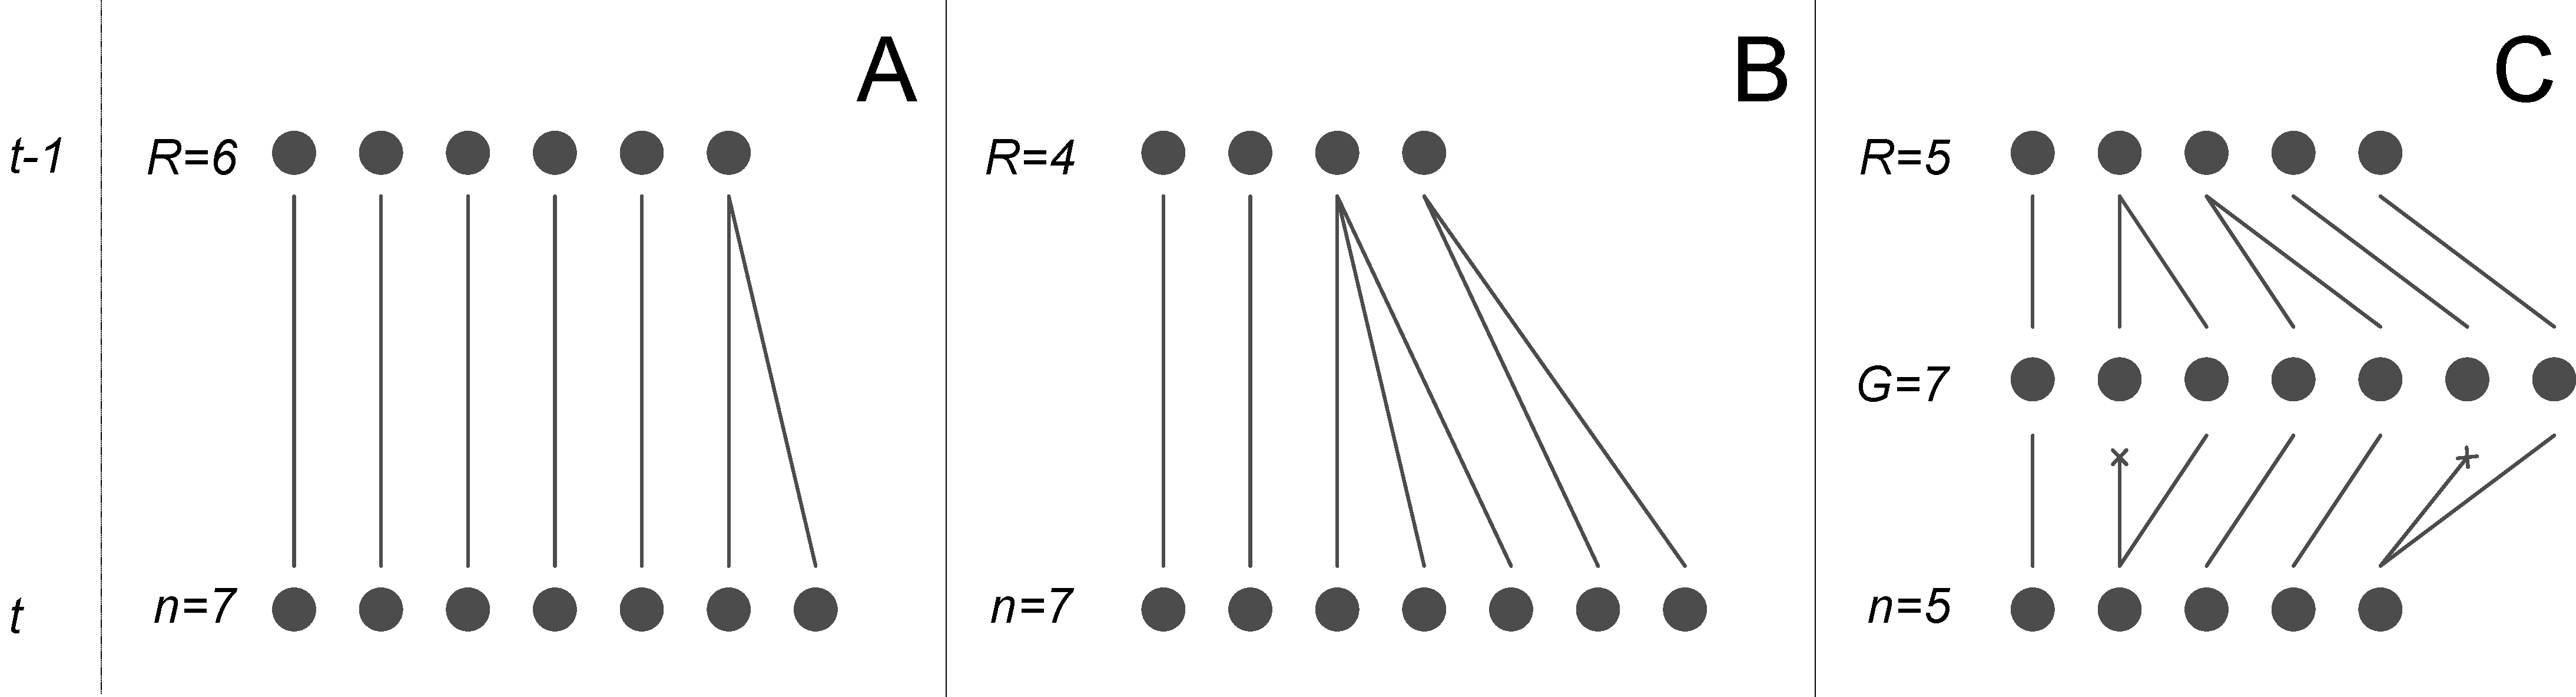
\includegraphics[width=1.0\textwidth]{fig/schematic.pdf}
  \caption{\label{fig:schematic} Realizations of sampling parental lineages under neutrality (A) and
    selection (B). \textbf{A} Under neutrality, possible coalescent events imply that number of
    parental lineages $n_p$ at $t-1$ is less than or equal to $n_o$ offspring lineages at $t$.
    \textbf{B} With selection, we add an intermediate gamete $n_g$ generation at $t-\frac{1}{2}$.
    Production of gametes is neutral, so $n_p\le n_g$. Gametes are sampled with rejection into
    offspring, so $n_o \le n_g$. Rejected samples shown with red crosses. $n_p$ - parental sample
    size (at $t-1$), $n_g$ - number of gametes (at $t-\frac{1}{2}$), $n_o$ - offspring (current)
    sample size (at $t$).}
\end{figure}

%In the Kingman coalescent, only a single coalescent event is allowed per generation, in
%approximation that sample size is much smaller than the population size: $n_o \ll N$. This implies
%that under neutrality $n_p \in [n_o-1, n]$. However, \citet{BhaskarEtAl2014} show that with
%increasing sample size, higher order coalescent terms contribute more substantially. This means that
%to describe the sample of size $n_o$, we need to consider $n_p$ potentially in the range
%$n_p \in [1, n]$.

In this selection model, the number $n_p$ of distinct parental lineages drawn is $n_p = n_o+n_r-n_c$, with $n_r$ 
the number of rejections and $n_c$ the number of coalescences. 
Thus $n_p$ can be smaller than $n_o$ (if there is more drift than selection), or larger 
(if there is more selection than drift). 




To express the allele-frequency spectrum $\afs{n_o}{t}$ in a sample size $n_o$ at time $t$ in terms of the parental AFS $\afs{n_p}{t-1}$, we take advantage of the exchangeability of the parents in the drawing process. If we perform the Wright-Fisher sampling sequentially, one offspring at a time, the order in which (previously unsampled) parental lineages are drawn is random. 
That is, we could have selected a random permutation of the parental population prior to starting the sampling process,
and decided to sample new parental lineages in order from this permutation. 
We can therefore condition on the random result of this permutation. 

The probability that we draw $i$ derived alleles in the offspring can be written as a sum over two intermediate random variables: 
the number $n_p$ of  distinct parental lineages drawn, and the number $j$ of derived parental lineages in a random sample of $n_p$ 
parental lineages. The event $r(j,n)$ that we draw $j$ derived alleles in a random sample of $n$ parental 
lineages has probability $P(r(j,n)) =\afs{n}{t-1}(j).$ We can therefore write


$$\afs{n_o}{t}(i) = \sum_{n_p,j} P(i,n_p,r(j,n_p)) =\sum_{n_p,j}  P(i,n_p | r(j,n_p)) \afs{n_p}{t-1}(j).$$
 

\sgcomment{Alternative derivation:
To estimate the allele-frequency spectrum $\afs{n_o}{t}$ in a sample size $n_o$ at time $t$, 
we can sum over the random variables $n_p,$ the number of distinct parental lineages selected, and $j$ 
the number of derived lineages among them:
 $$\afs{n_o}{t}(i)=\sum_{n_p,j} P(i,j,n_p) =  \sum_{n_p,j} P(i | j,n_p) P(j,n_p) $$
The event $(j,n_p)$ means that our Wright-Fisher sampling for $n_o$ offspring selected exactly $n_p$ distinct ancestors, 
of which $j$ are derived. 
If we perform the Wright-Fisher sampling sequentially, one offspring at a time, the order in which (previously 
unsampled) parental lineages are drawn is random. That is, we could have performed a random permutation of the 
parental population prior to starting the sampling process, and sampled new parental lineages in order from this permutation.  
Thus the event $(j,n_p)$ can be reformulated as the the joint events that the first $n_p$ parental alleles from the random 
permutation carry $j$ derived alleles and that exactly $n_p$ distinct parents were drawn in the Wright-Fisher sampling of the first $n_o$ 
offspring. Let $r(j,n_p)$ be the event that the first $n_p$ parental alleles from the random permutation carry $j$ derived alleles. Then $P(r(j,n_p)) =\afs{n_p}{t} )j),$ and we can write
$$\afs{n_o}{t}(i)=\sum_{n_p,j} P(i | r(j,n_p), n_p)  P(n_p | r(j,n_p) ) P(r(j,n_p)) = \sum_{n_p,j} P(i,n_p | r(j,n_p))  \afs{n_p}{t}$$
 \sgcomment{check if AFS is defined as probability or counts, in which case there is a scaling factor} where $r(j,n)$ is the event that $j$ out of the first $n$ sampled alleles in the population are derived. $r(j,n_p)$ follows a hypergeometric distribution and is distinct from $j$, the event of drawing $j$ parental derived alleles in the Wright-Fisher sampling process for the first $n_o$ offspring.
In words, the probability that we draw exactly $n_p$ parental alleles, of which $j$ are derived, is equal to the probability that a random subset of $n_p$ alleles drawn from the ancestral population contains $j$ derived alleles, times the probability that we draw exactly $n_p$ parental samples in that case.
Thus we can write
 \begin{equation}
\label{eq:recur}
 \afs{n_o}{t}(i)= \sum_{n_p=1}^{n_{p,max}} \sum_{j=0}^{n_p} P(i, n_p | r(j,n_p)) \afs{n_p}{t-1}(j).
\end{equation}
}

Under neutral evolution, $n_{p,max}\leq n_0$. Since we can obtain smaller AFS from larger AFS through downsampling (i.e., $\afs{n'}{t}  = P_{n',n} \afs{n}{t}$ for hypergeometric projection matrix \sgcomment{We need to use a variable other than $P$ for all these matrices and probabilities :)} $P_{n',n}$ and $n'<n$ )  \eqref{eq:recur} provides a closed form recursion for $\Phi_{n_o}.$ 
This property was used in \cite{JouganousEtAl2017} to efficiently compute distributions of allele frequencies under the large sample size limit.  

Under selection, $n_{p,max}$ can be larger than $n_o$, leading to an infinite set of coupled equations. A jackknife approximation can be used to simulate the drawing of additional lineages while preserving closure.
\cite{JouganousEtAl2017} also derived approximate recursion equations under selection, but these required multiple approximations: because Jouganous et al worked in a limit where the number of coalescent and selection events per generation is much smaller than one, every selective event led to $n_p> n_o,$ requiring a closure approximation.  
Our goal here is to take advantage of the fact that selective events can be treated exactly in the large sample size limit as long as  $n_p > n_o$ or,  equivalently, as long as  $n_s - n_d \leq 0.$
 
 
%   
%
%
%
%
%
%Under neutrality (Fig. \ref{fig:schematic}A), we have $n_p \in [1, n_o]$, therefore:
%
%\begin{align}
%  \label{eq:op-neutral}
%  \afs{n_o}{t} = \sum_{n_p=1}^{n_o}\mathcal{D}_{n_p\ra n_o} \afs{n_p}{t-1}
%\end{align}
%
%where $\mathcal{D}_{n_p\ra n_o}$ is a sparse matrix whose $i,j$th entry represents the 
%probability that... 
%
%
%
%
%This equation is closed with respect to the sample size $n_o$. 
%
%To include the effect of selection, we consider first the production of gametes from the parental
%generation as a neutral process. Changing the subscripts in \eqref{eq:op-neutral} to refer to Fig.
%\ref{fig:schematic}B, we have:
%
%\begin{align*}
%  \afs{n_g}{t-\frac{1}{2}} = \sum_{n_p=1}^{n_g}\mathcal{D}_{n_p\ra n_g} \afs{n_p}{t-1}
%\end{align*}
%
%Then, the produced gametes are sampled with rejection into $n_o$ offspring: \sgcomment{I don't understand how you get the next expression, logically}
%
%\begin{align*}
%  \afs{n_o}{t} = \sum_{n_g=n_o}^{\infty}\mathcal{S}_{n_g\ra n_o} \afs{n_g}{t-\frac{1}{2}}
%\end{align*}
%
%Combining the two expressions above, we get:
%
%\begin{align}
%  \label{eq:op-selection}
%  \afs{n_o}{t} = \sum_{n_g=n_o}^{\infty} \sum_{n_p=1}^{n_g} \mathcal{S}_{n_g\ra n_o}  \mathcal{D}_{n_p\ra n_g} \afs{n_p}{t-1}
%\end{align}
%
%Since we need to consider a potentially infinite number of gametes produced ($n_g$), the equation
%\eqref{eq:op-selection} is no longer closed with respect to sample size.
%
%Using $n_g=n_o+n_r=n_p+n_c$, we can re-write the above as:
%
%\begin{align}
%  \label{eq:op-selection}
%  \afs{n_o}{t} = \sum_{n_r=0}^{\infty} \sum_{n_c=0}^{n_o+n_r-1} \mathcal{S}_{(n_o+n_r) \ra n_o} \mathcal{D}_{(n_o+n_r-n_c)\ra (n_o+n_r)} \afs{n_o+n_r-n_c}{t-1}
%\end{align}
%
%This shows that the allele frequency spectrum in a sample size $n_o$ at present is a function of the
%AFS in the previous generation, with the sample size $n_o+n_r-n_c$.
%
%\ikcomment{I don't like this explanation, since I feel that the equation doesn't add much to the
%  figure.}
%

In the large population size and weak selection limit, the probability of observing a coalescence event 
in a generation is $\frac{n_o(n_o-1)}{2 N},$ whereas the probability of observing a selection event is
$2 n_o f_p s,$ with $f_p$ the parental deleterious allele frequency. These rates are familiar from the 
ancestral selection graph  \citep{KroneNeuhauser1997}. 
Since the probability of coalescence events grows quadratically with the sample size and the 
rate of selective events grows linearly, we expect  more drift events than selective events when 
$n_o>2Nf_p s.$ 






%The relative rates at which drift and selection events occur is familiar from coalescent theory,
%where the ancestral selection graph (\textit{ASG}) has rates of selective and drift events equal to
% \citep{KroneNeuhauser1997, Wakeley2009} with the number of lineages growing changing as
%
%\begin{align}
%  \label{eq:asg-size}
%  n \ra \begin{cases}
%    n+1 & \text{at rate } \frac{2 N s n}{2 N} ~ \text{ (selection) }\\
%    n-1 & \text{at rate } \frac{n(n-1)}{2 N}   ~ \text{ (coalescence) }
%  \end{cases}
%\end{align}
% \ikcomment{The reason I use continuous time rates here is that the coalescent term is obviously
%   quadratic in $n$. If I use discrete generations, it will be $\frac{\sigma}{\sigma+n-1}$ for
%   selection, and $\frac{n-1}{\sigma+n-1}$ for neutrality, which is a little less obvious.}

%The coalescence term is quadratic with respect to the sample size $n$, while the selection term is
%linear. The rate of coalescence is higher than the rate of selective events if the number of
%lineages $n>2Ns+1$.If $n$ is larger than $2 N_s$, we expect the number of lineages to decrease 
%more often than it increases.   

Our goal is to obtain an explicit recursion from equation \eqref{eq:recur} and show that its asymptotic
 behavior for large $n_o$ allows for almost-exact solutions even in the strong selection regime. 
 To do so, we will need to account for multiple coalescent events, which will require some careful bookkeeping.

%Our goal is to further investigate the interplay of selection and drift, and their effect on the
%\textit{AFS}. First, we propose a construction that allows us to calculate the \textit{AFS} under
%strong selection and large sample size, accounting for high-order coalescent terms. Second, we show
%that with increasing sample size, the system becomes asymptotically closed. We construct exact and
%approximate probability distributions that describe the number of contributing lineages.
%Additionally, we derive a normal approximation that allows us to calculate the quantile function of
%the sample size for a desired degree of closure.




\subsection{Constructing the transition matrix}

We can write Equation \eqref{eq:recur} in matrix form as \sgcomment{placeholder notation}
 \begin{equation}
\label{eq:recur}
 \afs{n_o}{t} = \sum_{n_p=1}^{n_{p,max}} \mathbf{P}_{n_p,n_o} \afs{n_p}{t-1}.
\end{equation}

Given that a sample of $n_p$ parents from the parental population has $j$ derived alleles ,the $(i, j)^{th}$ entry of $\mathbf{P}_{n_p,n_o} $ can be interpreted as the probability that Wright-Fisher sampling of $n_o$ offspring draws exactly $n_p$ parents, and that the offspring has exactly $i$ derived alleles. 
In the multiple-coalescence and strong selection regimes, we were unable to obtain an analytical expression
 that accounts for all the combinatorial ways to achieve this. 
 
 However, we can obtain fairly simple recursions in terms of the sample size $n_o.$ 
 Intuitively,  $\mathbf{P}_{n_p,n_o-1}$ provides information about the first $n_o-1$ 
 offsprings and the parental samples. 
 We can then draw an additional offspring, and update the transition matrix by summing over a 
 small number of coalescence and selection possibilities for that offspring lineage.  
 The derivation itself is somewhat tedious, and presented in Appendix X. 

 
  \sgcomment{Perhaps include description of recursion, jackknife, and convergence?}
 \section{Results}
\label{sec:results}
 
 




\subsection{Markov process construction}
\label{subsec:markov}
%
%\sgcomment{explain why we need a Markov process construction (do we need it?)}
%An alternative way to describe the time-evolution of the \textit{AFS} \eqref{eq:op-selection}, is to
%consider a single transition-probability matrix, $\mathbf{P}$, that describes the change due to
%drift and selection as a single term, and explicitly models derived and ancestral states:
%
%\begin{equation}
%  \label{eq:app:time-evolution}
%  \afs{n_o}{t} = \mathbf{P} \afs{n_o}{t-1}
%\end{equation}
%\sgcomment{why is this closed? Should the RHS be $n_p?$}
%
%\ikcomment{$n_o$ and $n$ (without subscript) are the same thing. I use $n_o$ explicitly everywhere,
%  but I can probably drop the subscript when it's clear from context.}
%
%$\mathbf{P}$ is a square $n_o \times n_o$ matrix, and it enumerates the number of derived alleles
%($i$) at a biallelic locus in a sample of size $n_o$. $\mathbf{P}$ includes contributions from
%all possible configurations of parents $n_p$, weighted by the probability of the relevant
%coalescent/selective event. We will need to keep track of sample size and number of derived alleles
%in the offspring ($o$) and parents ($p$) lineages for a given generation. For example, we use
%$\Dfrac{i_p}{n_p}$ (read as ``$i_p$ out of $n_p$'') to denote a sample of size $n$ with $i$ derived in
%the parental generation (at $t-1$).
%
%Instead of using the summation formulation presented in \eqref{eq:op-selection}, we use recursive
%conditional probabilities, where transitions are defined in terms of transitions in smaller
%sample sizes. Each entry of the matrix, $\mathbf{P}_{(i_o,i_p)}$ is a a transition probability from
%$i_p$ to $i_o$ derived alleles with sample sizes $n_p$ and $n_o$, respectively. The key observation
%is that to construct such probabilities, we can condition on a set of coalescent events
%$\{\Lambda\}$ in a smaller sample size:
%
%\begin{align*}
%  \label{eq:coal-recursion}
%  \mathbf{P}_{(i_o,i_p)} &= P\left[\Dfrac{i_o}{n_o} \cond \Dfrac{i_p}{n_p}\right] \\
%  &= \sum_{\lambda\in\{\Lambda\}}P(\lambda)
%  P\left[\Dfrac{i_o}{n_o} \cond \Dfrac{i_p}{n_p},\lambda\right] \\
%  &= \sum_{\lambda\in\{\Lambda\}}P(\lambda)
%  P\left[\Dfrac{i_o-|\lambda|_{i_o}}{n_o-|\lambda|_{n_o}} \cond \Dfrac{i_p-|\lambda|_{i_p}}{n_p-|\lambda|_{n_p}}\right]
%\end{align*}
%
%Above, $|\lambda|$ denotes the size of the coalescent event. The third equality ascertains that
%conditioning on a coalescent event is equivalent to subtracting relevant lineages from the sample.
%This yields a recurrence where transition probabilities in a sample of size $n$ can be
%described recursively in terms of transition probabilities in smaller sample sizes, $n' \in [1, n-1]$.
%
%The full derivation of $\mathbf{P}$ for neutral and $\mathbf{P}_s$ for selective cases can be found
%in the appendix. This involves enumerating all the coalescent and selective events between samples of
%different sizes. We avoid it here for brevity.

The maximum sample size is $n=N$, the size of the entire population. We expect that in the regime
where $n\ll N$, the calculations with the present model do not differ substantially from the
prediction under the standard coalescent, or \citep{JouganousEtAl2017}. In the limit where
$n \ra N$, we expect the transition probabilities in $\mathbf{P}_s$ to approach those in the full
Wright-Fisher model (\textit{i.e.} \cite[eq. 1.58]{Ewens2004}).

Similar to \eqref{eq:op-selection}, the transition probability matrix with selection
($\mathbf{P}_s$), involves considering a large number of intermediate lineages. In practice, we
limit the number of selective events to at most one per lineage -- which means that the maximum
number of contributing lineages is $2n_o$ -- one selective death for each offspring. This allows us
to model strong selection, while limiting the number of coalescent configurations we need to
consider when building $\mathbf{P}_s$. While it should in principle be possible to include
additional selective events, we do not pursue this here.

The above restriction implies that under strong selection with large number of derived lineages $i$,
there is a possibility that some probability is \textit{missing} from $\mathbf{P}_s$. However, since
this model forms a proper Markov chain, we can calculate the total missing probability, by
subtracting the total probability for a given derived allele count $i$ from $1$. This gives a rather
natural proxy to checking how many extra lineages are required by selection. As we show further,
this missing probability tends to $0$ with increasing sample size.

The recursive nature of these calculations makes them relatively inefficient. Using a dynamic
programming algorithm, we implement the construction of the neutral matrix $\mathbf{P}$ in the order
of $O(n^3)$ operations. The selection transition probability matrix $\mathbf{P}_s$ needs $O(n^4)$
operations, due to the need to consider intermediate lineages. The increase in complexity makes this
approach unsuitable for large sample sizes, but we derive several approximations in the following
sections.

\subsection{Calculation of allele frequency spectra}
\label{subsec:afs}

Once the truncated matrix $\mathbf{P}_s$ is constructed, it can be used to calculate the allele
frequency spectrum. For example, in the infinite sites model at equilibrium, we can approximate the equilibrium
\textit{AFS} $\Phi$ as a solution to a linear system:

\begin{equation}
  \label{eq:sfs-calc}
  \Phi = \Phi Q + n \mu e_1
\end{equation}
where $\mu$ is the per-site mutation rate, and $e_1$ is the first column of the identity matrix of
size $n$. Figure \ref{fig:strong-selection} shows the comparison of the \textit{AFS} calculated from
Equation \eqref{eq:coal-recursion, eq:sfs-calc}, the diffusion approximation \cite[eq.
9.23]{Ewens2004}, and the calculation performed in \texttt{Moments} \citep{JouganousEtAl2017}.
Panels A and B show the \textit{AFS} under neutrality, C and D under strong negative selection.
Under neutrality, all the models agree, yeilding similar \textit{AFS}. When the sample size is equal
to the population size (Fig. \ref{fig:strong-selection}B), we also include the \textit{AFS} from the
full Wright-Fisher model, which the other three calculations agree with.

Figure \ref{fig:strong-selection}C shows a comparison at strong negative $Ns=50$, with the population
size ($N=1000$), which is substantially larger than the sample size ($n=100$). There is a small
deviation between the approaches at large allele frequencies. At stronger selection coefficients,
\texttt{Moments} suffers from numerical instability, while the diffusion approximation performs
well.

If the sample size is the same as the population size ($n=N=100$) (Fig.
\ref{fig:strong-selection}D), the diffusion approximation and \texttt{Moments} perform detract \sgcomment{departs?} from
the Wright-Fisher prediction. The approach presented here (\ref{eq:coal-recursion}) shows a better
match to the Wright-Fisher model at small allele frequencies, but deviates later. We believe that
the disagreement is due to the fact that we only allow at most one selective event per lineage,
while there is no such limitation in the Wright-Fisher model.

\begin{figure}
  \centering
  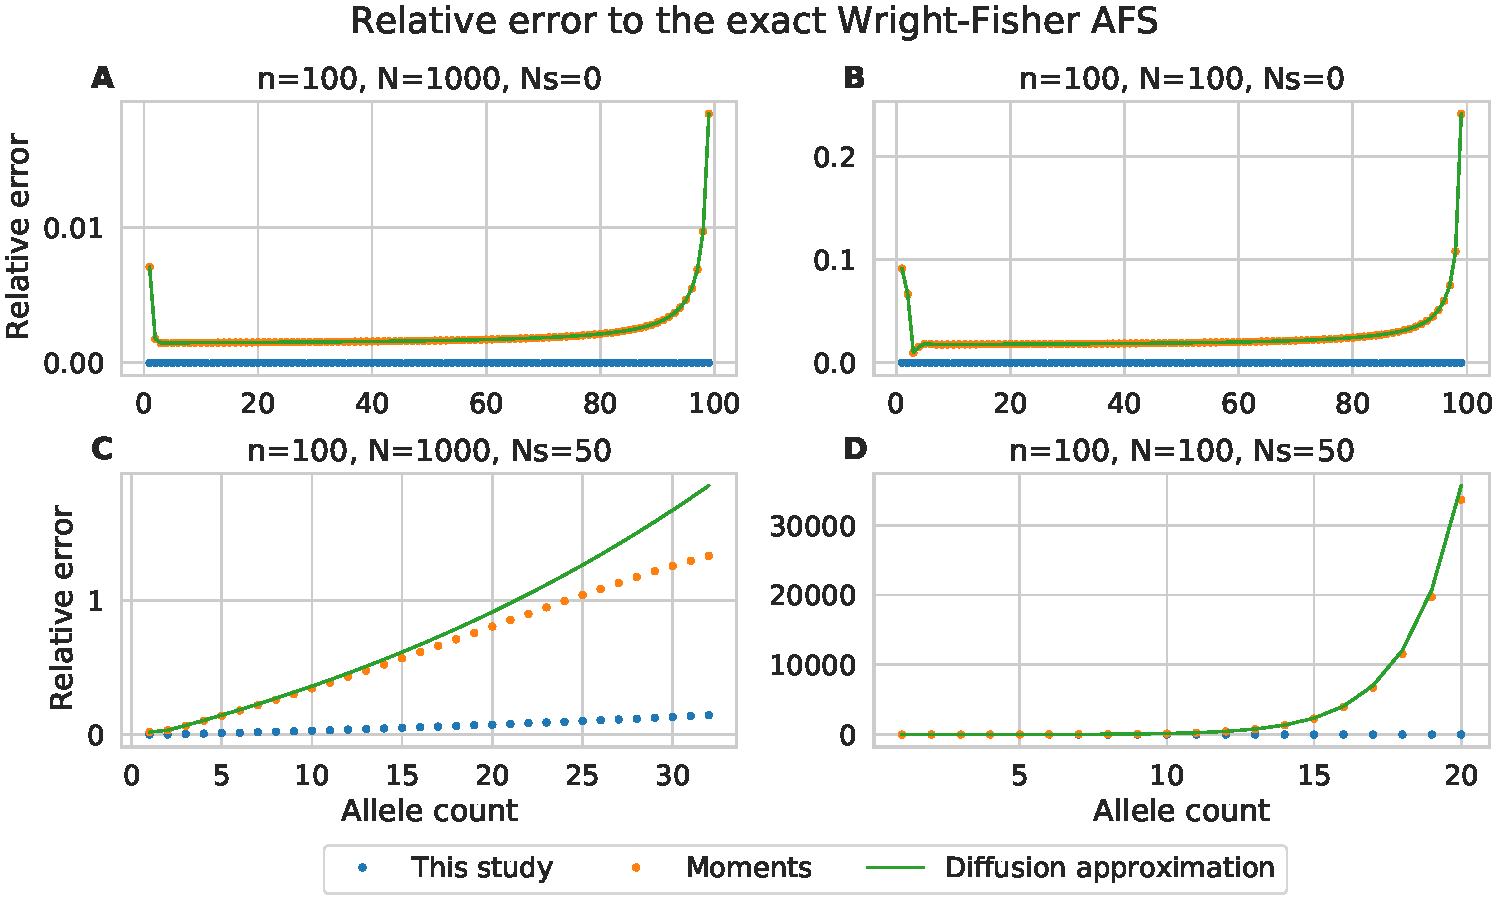
\includegraphics[width=0.7\textheight]{fig/strong_selection_four_panel.pdf}
  \caption{Normalized allele frequency spectra in a sample of size $n=100$, for highly deleterious
    alleles ($Ns=50$). (A) shows the frequency spectrum in a sample from a large population
    ($N=1000$), (B) in a small population ($N=100$). \sgcomment{The caption does not correspond to the figure.
    what is going on with the stripes? Presumably some log artefact? Maybe clarify that "numeric" is this work. Since the genome is only $3\times10^9 bases$, it would make sense to cutoff at $10^-9$. Would also highlight differences better. Axis labels missing. PErhaps put the x label in proportions, and cut off for strong selection?}
    \label{fig:strong-selection}
   }
 
\end{figure}


\subsection{Closure properties}
\label{subsec:closure}

To investigate the closure properties of $\mathbf{P}_s$, we can calculate the total probability that
more that $n_o$ parental lineages contribute to a sample of size $n_o$. \sgcomment{I'm not sure
 I understand what you describe below. My take:}
Since $P_{n_o,n_p}(i,j)$ is a probability distribution over $n_p$ and $i$, we can easily compute the probability lost to 
truncation as $1-\sum_{i=0}^{n_o} \sum_{n_p=0}^{n_o}{P_{n_o,n_p}(i,j)}$. 


By construction, the sum
of rows of $\mathbf{P}_s$ should correspond to the total probability mass that included
configurations contribute (Fig. \ref{fig:rec-selection}). Thus, the probability that some number of
configurations are unaccounted for, with $j$ derived alleles in the parental sample, is given by
$1-\sum_{i=0}^{n}\mathbf{P}_s(i,j)$. This probability depends on the number of derived alleles
carried by the parental sample: the more derived alleles, the higher the likelihood of a selective
event. Figure \ref{fig:missing} shows the probability of missing configurations in a sample size of
$n=200$ in the worst-case scenario, with $j=200$ derived lineages.

\begin{figure}
  \centering
  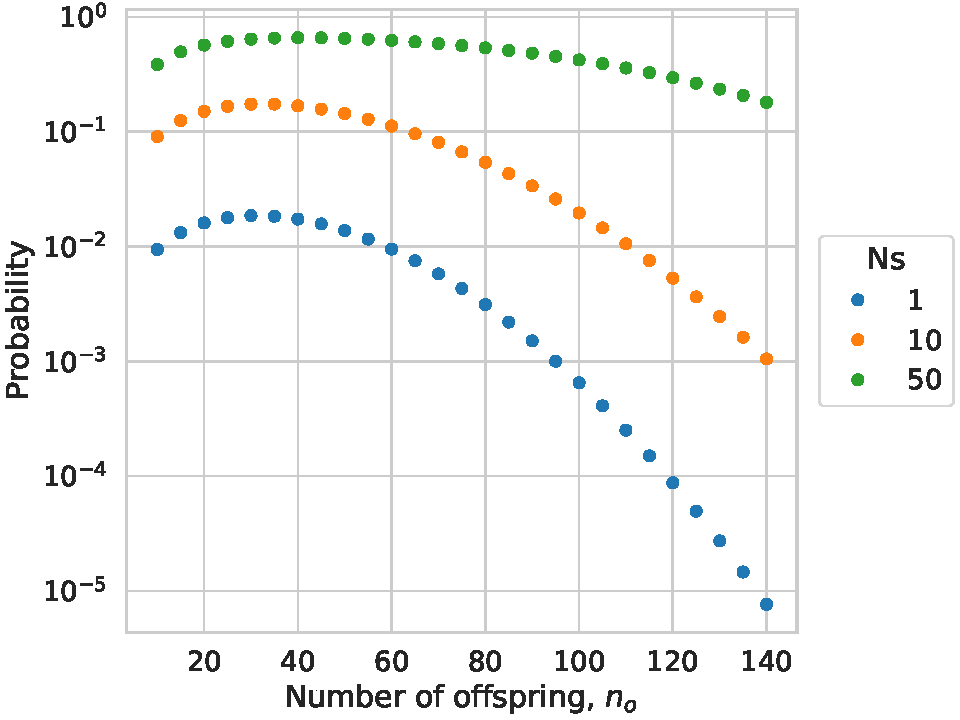
\includegraphics[]{fig/missing.pdf}
  \caption{Probability that unaccounted lineages contribute to the transition probabilities. The
    probabilities are calculated as 1 minus the sum of probabilities for the state where every
    allele is derived.}
  \label{fig:missing}
\end{figure}

Since the expected number of drift events increases quadratically and the number of selective events
increases only linearly, the probability that we need additional lineages decreases rapidly with
sample sizes.

\section{Asymptotic closure properties}

We now want to determine what sample size is sufficient so that the number of coalescent events due
to drift is almost always larger than the number of selection events, such that the system remains
closed \eqref{eq:op-selection}. We derive several approximations to the model proposed in the first
section, in order to get a better understanding of this behavior.

In the following derivations, we are assuming that the derived allele is present at frequency $x$,
as opposed to explicitly modeling the count of derive alleles \ref{sec:markov}, which simplifies the
calculations. When looking for the upper bound on the number of rejected lineages, we take $x=1$,
since only derived alleles experience selection.

\subsection{Mean number of contributing lineages}
\label{sec:mean-contr}

For a given sample size, the probability that $n_p$ parents have contributed is:

\begin{align}
  \label{eq:conditional}
  Pr(n_p | n_o) = \sum_{n_g} Pr(n_p | n_g)Pr(n_g | n_o)
\end{align}

Where $n_p$ and $n_g$ is the number of contributing parents and gametes, respectively (Fig.
\ref{fig:schematic}B). Note that we consider this backward in time, so $n_o$ is given, and we ask
the probability of $n_p$ conditional on $n_o$.

As a first order approximation, we can model the expectation $E[n_p | n_o]$ as the sum of lineages
used under drift $\tilde{E}[n_p | n_o]$ (Fig. \ref{fig:schematic}A) plus the number of extra
lineages required by selection, $E[n_r | n_o]$.

\begin{equation*}
  \begin{aligned}
    \label{eq:lineages-approx}
    \hat{E}[n_p  | n_o] &= \tilde{E}[n_p | n_o] + \hat{E}[n_r | n_o] \\
    &= N\left[1-\left( 1 - \frac{1}{N} \right)^n \right] + n\left( \frac{xs}{1-xs}\right) \\
    &\underset{N\gg n}{\approx} \frac{nxs}{1-xs} - \frac{n^2}{2N}
  \end{aligned}
\end{equation*}

The expectations can be derived directly or from the corresponding probability distributions
\ref{subsec:distribution}.The second approximation is made under the assumption that the sample size
is much smaller than the population size. The increase of the number of lineages due to selection is
linear. Drift decreases the number of lineages as a quadratic term with respect to the sample size.
This is analogous to the results from the ancestral selection graph \citep{KroneNeuhauser1997}, eq.
\eqref{eq:asg-size}. Solving \eqref{eq:lineages-approx} for $n_o^* > \hat{E}[n_p | n_o]$ yields:

\begin{equation}
  \label{eq:critical-sample}
  n_o^* \ge 2Nxs
\end{equation}

This represents a critical sample size, above which drift outpaces selection.
Note again the similarity to \eqref{eq:asg-size}.

Figure \ref{fig:critical-sample-size} shows the critical sample size for several selection
coefficients, assuming the entirety of the sample is derived ($x=1$) in a population of $N=1,000$.
The $Y$ axis shows the fraction of contributing parental lineages to the sample size,
$\frac{n_p}{n_o}$. Above the horizontal line $\frac{n_p}{n_o} > 1$, selection dominates. Below,
drift reduces the number of used lineages. The intercept of the line with $\frac{n_p}{n_o} = 1$ is
the critical sample size, which is well-approximated by $2Nsx$.

\begin{figure}
  \centering
  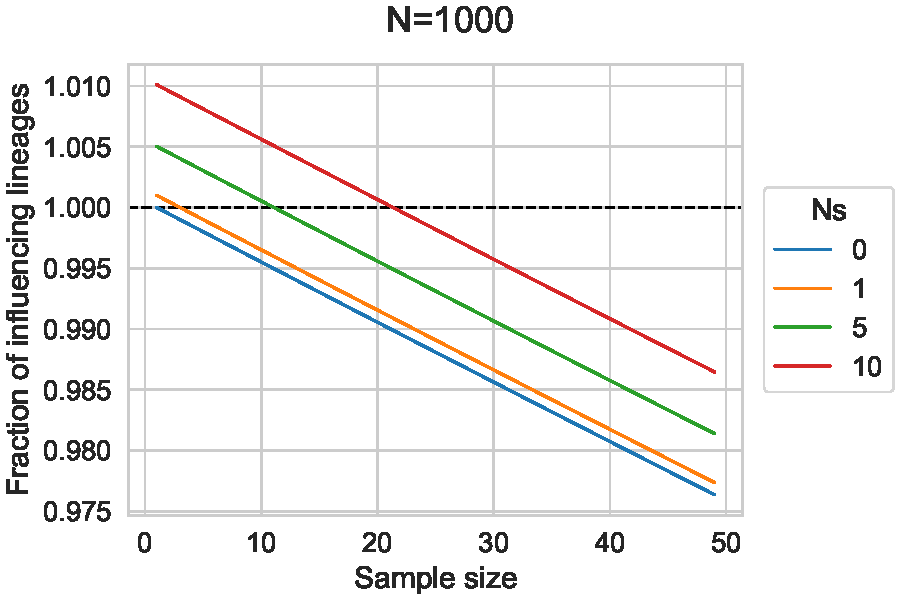
\includegraphics{fig/critical_sample_size.pdf}
  \caption{Critical sample size for different selection coefficients. The $Y$ axis shows the
    fraction of parental lineages over the sample size, $\frac{n_p}{n_o}$, each line corresponds to a
    different selection coefficient. Above $\frac{n_p}{n_o}\ge 1$, selection dominates, below -- drift.
    The critical sample size, where the expected number of parental contributing lineages is smaller
    than the sample size is well-approximated by $2Ns$.}
  \label{fig:critical-sample-size}
\end{figure}

\subsection{Distribution of number of contributing lineages}
\label{subsec:distribution}

We now construct a probability distribution of the number of contributing lineages one generation
into the past \ref{fig:schematic}B, \eqref{eq:conditional}. 

The number of parental lineages used by drift can be modelled by the modified occupancy
(Arfwedson) distribution \citep{Wakeley2009,ONeill2019,JohnsonEtAl2005}. This is given by:

\begin{align}
  \label{eq:occupancy}
  P(n_p|n_g) = \frac{S_2(n_g,n_p) N!}{(N-n_p)! N^{n_g}}
\end{align}
where $S_2(n_g,n_p)$ is a Stirling number of the second kind, which is the number of ways to partition
$n_g$ gametes into $n_p$ parents (see \cite{JohnsonEtAl2005} section 10.4 for a thorough treatment).
Note that the under drift, the number of parents will be smaller or equal to the number of gametes
$n_p \le n_g$.

The distribution of the number of gametes, $n_g$ is given by the negative binomial, parameterized by
probability of resample $s$, and the total number of trials before $n_o$ successes (\textit{i.e.}
$n_r+n_o$):

\begin{align}
  \label{eq:neg-binomial-trials}
  P(n_g|n_o) = \binom{n_g-1}{n_o-1}(1-xs)^{n_o}(xs)^{n_g-n_o}
\end{align}

Here, the number of gametes can be larger that the sample size $n_o \le n_g$, if selection is present.

Combining the two distributions together through \ref{eq:conditional}, we get:

\begin{align}
  \label{eq:lineages-in-past}
   Pr(n_p|n_o) = \sum_{n_g=1}^{\infty} \frac{S_2(n_g,n_p) N!}{(N-n_p)! N^{n_g}} \binom{n_g-1}{n_o-1}(1-xs)^{n_o}(xs)^{n_g-n_o}
\end{align}

This distribution does not appear to have a simple analytical form. However, it can be computed
efficiently using methods presented in \citep{ONeill2019}. Figure \ref{fig:sampling-dist} shows the
distribution of the number of contributing parental lineages for several selection coefficients for
a sample $n=20$. In the absence of selection, the distribution has zero probability above $n=20$, as
no extra lineages can be sampled. As the strength of selection is increased, we begin requiring
larger number of lineages.

\begin{figure}
  \centering
  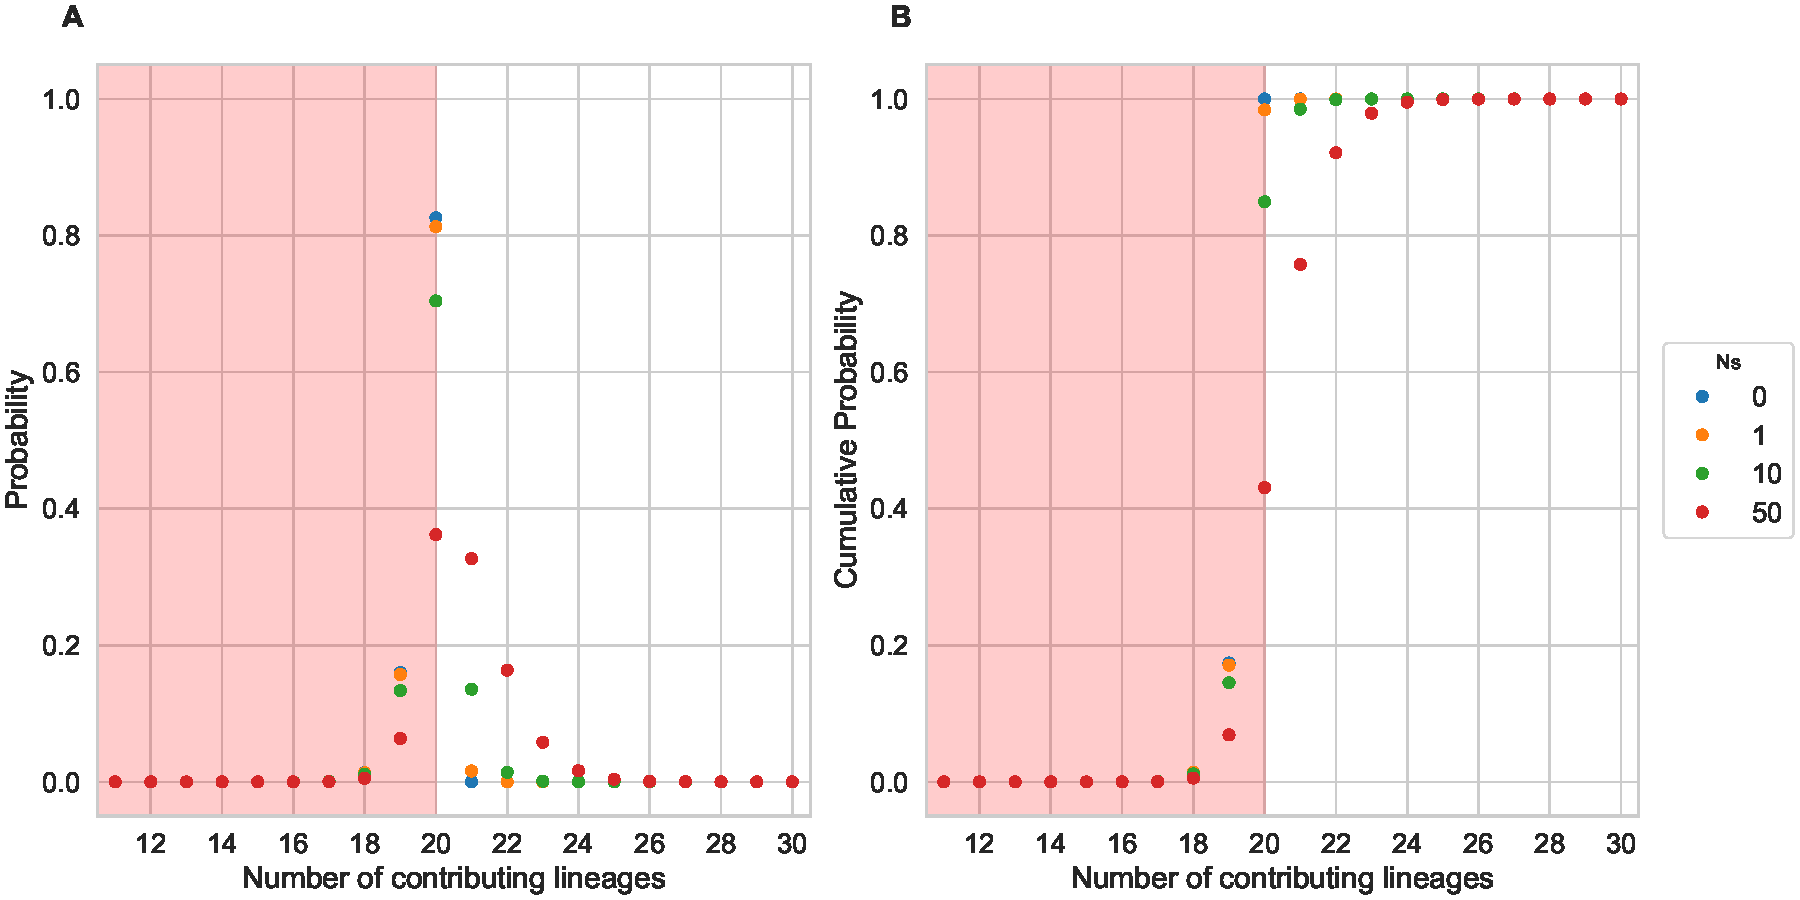
\includegraphics[width=\textwidth]{fig/distributions.pdf}
  \caption{\textbf{A} The distribution and \textbf{B}, cumulative distribution of the number of
    parental contributing lineages one generation into the past ($n=20$, $N=1000$). Shaded red area
    shows the drift-dominated regime, where the number of lineages is smaller than the sample size.}
  \label{fig:sampling-dist}
\end{figure}

We defined the critical sample size as $n_o^* > E[n_p | n_o]$. However, the distributions in
\ref{fig:sampling-dist} show that there is a large probability that $n_p>n_o$ at $n_o^*=2n=20$. In
order to guarantee that drift will out-pace selection, we can calculate the cumulative distribution.
This implies that a sample size in which the \textit{majority} of lineages are accounted for can be
substantially larger than the critical sample size of equation \eqref{eq:critical-sample}. To derive
a convenient analytical approximation, we turn to the normal approximation in the next section.

\subsection{Normal approximation}

We can construct a normal approximation to the distribution of the number of contributing lineages.
This approximation will allow us to calculate sample size where, for example, the number of
contributing lineages is smaller that the sample size $95\%$ of the time, instead of $50\%$, as
given by $n_o^*$ in equation \eqref{eq:critical-sample}.

The occupancy distribution is approximated by the normal \citep{ONeill2019} when $n_o \ll N$.
Likewise, the number of failures ($n_r$) before a given number of successes, can be approximated by
the normal distribution. In the case of large population size, as required by the approximation of
the occupancy by the normal, we can approximate the total number of contributing lineages as the sum
of lineages contributed by the two distributions.

The random variable which is a sum of two normally-distributed random variables is also normal, with
$\mu=\mu_1+\mu_2$ and $\sigma^2 = \sigma^2_1 + \sigma^2_2$. By combining the required expectations
and variance, we find that the normal approximation then has the form:

\begin{align}
  \label{eq:normal-approximation}
  Pr(\mathcal{R}=r|n) \approx \mathcal{N}( \mu &= \left[(s n)/(1 - s) + N (1 - (1 - 1/N)^n)\right],\\
  \sigma &= \sqrt{N \left((N-1) \left(1-\frac{2}{N}\right)^n+\left(1-\frac{1}{N}\right)^n-N\left(1-\frac{1}{N}\right)^{2 n}\right)+\frac{n s}{(1-s)^2}})
\end{align}

Figure \ref{fig:normal-approximation} shows the quantiles of the normal approximation. We see that
up to $99\%$ of the lineages will be contained within the sample of 200 with $Ns=20$. Larger
percentiles will require larger sample sizes.

\begin{figure}
  \centering
  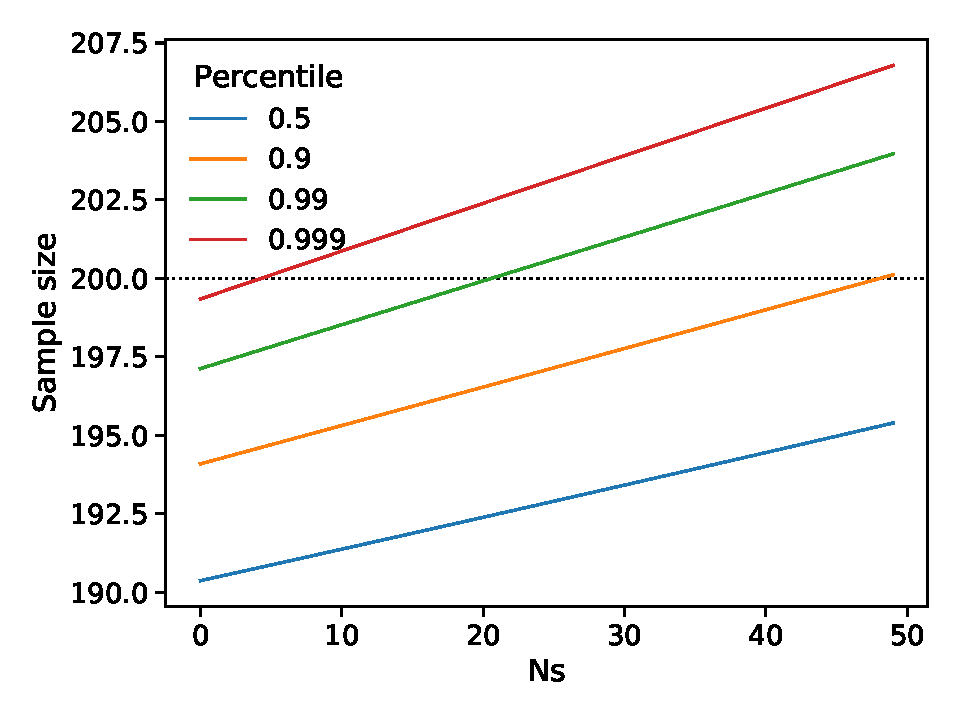
\includegraphics[]{fig/quantile.pdf}
  \caption{\ikcomment{TODO: need to resolve this still} The quantile function of the closure of the
    sample \eqref{eq:normal-approximation}. Each line corresponds to different percentile of the
    normal approximation. Black dashed line shows the reference sample size $n_o^*=200$
    \sgcomment{does it play a special role? If not why mention it (or have this line, really)?}.
    \sgcomment{It also seems like showing the cumulative distributions themselves would be more
      intuitive. E.g $\log(missing p)$. Also would be nice to have the numerical calculation. Could
      you get the cumulative distribution for the occupancy distribution from the Oneil algorithm? }}
  \label{fig:normal-approximation}
\end{figure}

\subsection{Integrating over few generations} 
To increase the chances that the number of lineages ancestral to a sample 
of size $n_o$ is less than $n_o$, we can also chose to compute a transition matrix over more 
than a single generation. In this case, lineages gained by selective death at one generation can 
can be compensated by loss to genetic drift at another generation. If the expected number of 
drift events is higher than the expected number of selective deaths, this can reduce the likelihood 
of chance events. Asymptotic results suggest ... 

Such transition matrices can also be computed iteratively. If  $n_g$ is the number of contributing 
lineages in the grandparental generation, and $k$ is the number of derived among those, and we define 
 $P(i, n_g | q(k, n_g))$, as above, as the probability of drawing $i$ derived alleles and using exactly $n_g$
 grandparental alleles given the event $q(k, n_g)$ $k$ of the first $n_g$ grandparental alleles are derived, we can 
 condition on the number of contributing alleles $n_c$ and the number of derived alleles $j$ among them in the parental generation:
 
 \begin{equation}
 \begin{split}
 P(i, n_g | r(k, n_g)) & = \sum_{j,n_c} P(i, n_g ; j, n_c r(j,n_c)  | q(k, n_g))\\
 &= \sum_{j,n_c} P(i, n_c,  r(j,n_c); n_g  | q(k, n_g))\\
 &= \sum_{j,n_c} P(i, n_c|   r(j,n_c); n_g  ; q(k, n_g))  P(r(j,n_c); n_g  | q(k, n_g))\\
 &= \sum_{j,n_c} P(i, n_c |   r(j,n_c))  P( r(j,n_c); n_g  | q(k, n_g))\\
 &= \sum_{j,n_c} P(i, n_c |   r(j,n_c))  P( r(j,n_c); n_g  | q(k, n_g))
 \end{split}
\end{equation}
and \sgcomment{despite the crap notation}, this is just the product of quantities we have already computed.


\section{Conclusion}
\label{sec:conclusion}

Classically, the coalescent considers models in the absence of natural selection. Since selection
can increase the number of contributing lineages back in time, the coalescent can no longer be
represented by trees, but instead acquires a graph structure. The ancestral selection graphs
\citep{KroneNeuhauser1997} deal with this in the limit of large population size ($N$).

The large population size approximation implies that the sample size $n$ is much smaller than the
whole population ($n \ll N$), so it is unlikely that more than one coalescent event will happen per
generation. However, recent work \citep{BhaskarEtAl2014,NelsonEtAl2019} pointed out that this
assumption is unreasonable with sample sizes pertinent to modern experiments. As a results, models
that consider multiple coalescent events per generation are gaining increased relevance in the
field \citep{FlemmingtonVoit}.

In this work we show that increasing the sample size has another unexpected consequence. As sample
size increases, the larger number of lineages needed due to selection can be masked by coalescent
events. In this sense, the large sample size rescues the model from effect of selection. This means
that recursion equations needed to calculate sample properties are asymptotically closed with large
population size.

At first approximation, $n_o^*=2Nsx$ is a critical sample size, where the decrease of lineages due to
coalescent back in time out-competes the increase due to selection (eq. \eqref{eq:critical-sample}).
Further, we derive the full probability distribution for the number lineages needed with given
selection coefficient and sample size (eq. \eqref{eq:lineages-in-past}). Unfortunately, the
distribution does not have a closed form, so we derive a normal approximation to the number of
lineages that contribute to a sample (eq. \eqref{eq:normal-approximation}). The normal approximation
then allows us to get a quantile function that we use to find if the model preserves closure with
some confidence level.

This work has several implications. First, we can combine the model described here with the
jackknife approximation \citep{JouganousEtAl2017}. This will allow us to construct a more robust
inference framework that can account for large sample size and strong selection.

Further, the results here suggest that effect of weak selection may be detectable in studies with
large sample sizes. This may open up a way for new investigations of natural selection in population
genetics.

\bibliography{disco}

\section{Appendix}
\subsection{Table of symbols}

\label{ssec:tab-symbols}
\begin{center}
\begin{tabular}{lll}
Symbol & Generation & Meaning\\
\hline
$p$ & $t-1$ & Parental generation\\
$c$ & $t-\frac{1}{2}$ & Contributing (intermediate, selection only)\\
$o$ & $t$ & Offspring (current) generation\\
\end{tabular}
\end{center}

\begin{center}
\begin{tabular}{ll}
Symbol & Meaning\\
\hline
$n$ & Sample size\\
$i$ & Number of derived alleles in sample $n_{\cdot}$\\
$\Dfrac{i}{n}$ & $i$ derived \emph{out of} $n$ total alleles\\
\end{tabular}
\end{center}

\subsection{Neutral case}

We want to construct the entries in the probability matrix
$P\left[ \Dfrac{\cdot}{n_o} \cond \Dfrac{\cdot}{n_p} \right]$ in terms transition probabilities in
smaller sample sizes. Under neutrality, the number of contributing parental lineages $n'_p$ (at
$t-1$) can not be larger than the number of offspring lineages $n_o$. Since $\mathbf{P}$ is square,
$max(n_p)=max(n_o)=n$. Thus, our aim is to express every entry of $\mathbf{P}$,
$P\left[ \Dfrac{\cdot}{n} \cond\Dfrac{\cdot}{n} \right]$, in terms of
$P\left[ \Dfrac{\cdot}{n-1} \cond \Dfrac{\cdot}{n-1} \right]$. Since we never require extra lineages
($n_p\le n_o$), the recurrence is closed.

To calculate the transition probabilities, we first condition on the state of the last parental
allele drawn, and then on the coalescent event that last offspring lineage participates in. The
recurrence is shown in figure \ref{fig:rec-neutral}. The panel on the right depicts the coalescent
event for each term. Empty circles represent ancestral alleles, filled circles -- derived. The
square box represents a sample of size $n-1$. The first three terms in the sum correspond to the
cases where the last parent that we drew was ancestral, last three -- derived.
\sgcomment{Would it be worth presenting the non-square transition probabilites as well to prepare the reader for what comes next with selection}

\begin{figure}
  \centering
  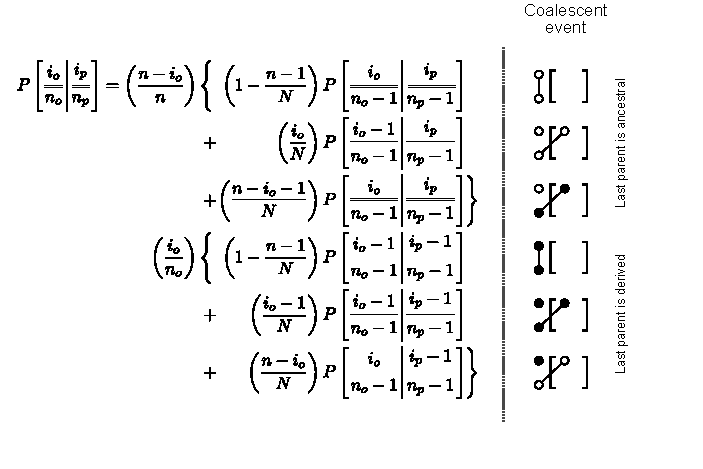
\includegraphics[width=0.9\textwidth]{fig/recurrence-neutral-annotated.pdf}
  \caption{Recurrence defining transition probabilities in a model without selection. Right panel
    shows coalescent events corresponding to each summand. Each transition probability is defined in
    terms of transition in a smaller sample size. First three terms are conditional on the last
    parent having an ancestral state, last three -- derived. Filled circles -- derived alleles;
    empty circles - ancestral alleles; square brackets -- sample of size $n-1$.}
  \label{fig:rec-neutral}
\end{figure}

When calculating a single entry in \ref{fig:rec-neutral}, the variables have the following ranges.
\begin{equation}
  \begin{aligned}
    n_p &= n \\
    i_p &\in [0, n] \\
    n_o &= n \\
    i_o &\in [0, n] \\
  \end{aligned}
\end{equation}

The recurrence is calculated while $n>1$, with the following base cases:
\begin{align*}
  P\left[ \Dfrac{1}{1} \cond \Dfrac{1}{1} \right] &= 1 \\
  P\left[ \Dfrac{0}{1} \cond \Dfrac{0}{1} \right] &= 1 \\
  P\left[ \Dfrac{0}{1} \cond \Dfrac{1}{1} \right] &= 0 \\
  P\left[ \Dfrac{1}{1} \cond \Dfrac{0}{1} \right] &= 0 \\
\end{align*}

\subsection{Selection case}

Due to selective deaths, the number of lineages ($n_c$) that contribute to the current generation
can be larger than the number of offspring ($n_o$), and especially so with strong
selection. Because the number of sampling configurations can be large, we use dynamic programming 
to estimate $\mathbf{P}_{n_p,n_o}$ by summing over the possibilities for the last successful draw. Using the
probability interpretation of the transition matrix, $\mathbf{P}_{n_p,n_o}(i,j) = P(i, n_p | r(j, n_p)),$ the
probability that we draw $i$ derived offspring and exactly $n_p$ parental offspring given that $j$ of the first
$n_p$ sampled parental alleles are derived.  The last successful draw event can be specified by the number $t \in \{0,\infty\}$ 
of prior failed draws due to selection since the last successful draw, the allele $a \in {A, D}$ selected, 
and the event $c$ of whether or not the sampled parental allele was previously drawn $c\in \{True, False\}$. We also consider the event $s \in \{True, False\}$ of whether the last draw was successful. Finally, let us define the event $E_{n_o,t}(i,n_p)$ that we have drawn 
$i$ derived offspring among $n_o$ successful draws followed by $t$ failures, and that this required exactly $n_p$ parental lineages.   
\begin{equation}
\begin{split}
P(i, n_p | r(j, n_p)) = P(E_{n_0,0}(i,n_p)  | r(j, n_p)) &=  \sum_{a, c,t} P(a,c,t; E_{n_o,0}(i,n_p)  | r(j, n_p)) 
 \end{split}
\end{equation}
Let us consider the term $a=A$, $c=False$ \sgcomment{We could use a better notation here, eg using tikz. }
\begin{equation}
\begin{split}
P(a=A,c=False,t; E_{n_o,0}(i,n_p)  | r(j, n_p)) &= P(a=A, c=False, t,s=True; E_{n_o,t}(i,n_p-1) | r(j, n_p))\\
&= P(a=A, c=False, t; E_{n_o,t}(i,n_p-1) | r(j, n_p))\\
&=P(a=A, c=False, t ; E_{n_o,t}(i,n_p-1); r(j, n_p-1) | r(j, n_p))\\
&=P(a=A, c=False, t ; E_{n_o,t}(i,n_p-1)| r(j, n_p-1)  r(j, n_p)) P(r(j, n_p-1) |  r(j, n_p))\\
&=P(c=False, t;  E_{n_o,t}(i,n_p-1) | r(j, n_p-1)  r(j, n_p)) \frac{n_p-j}{n_p}\\
&=P(c=False | t;  E_{n_o,t}(i,n_p-1) | r(j, n_p-1)  r(j, n_p)) P(t;  E_{n_o,t}(i,n_p-1) | r(j, n_p-1)  r(j, n_p)) \frac{n_p-j}{n_p}\\
&=\left(1-\frac{n_p-1}{N}\right) P(t;  E_{n_o,t}(i,n_p-1) | r(j, n_p-1)  r(j, n_p)) \frac{n_p-j}{n_p}\\
&=\left(1-\frac{n_p-1}{N}\right) P(t;  E_{n_o,t}(i,n_p-1) | r(j, n_p-1)) \frac{n_p-j}{n_p}
\end{split}
\end{equation}
where the fourth line uses Bayes rule, and  most other lines are exercises in rewriting the same event in different ways. 
Other combinations of $a$ and $c$ also yield expressions in terms of probabilities $P(t;  E_{n_o,t}(i,n_p) | r(j, n_p))$ for the state prior to the successful draw \sgcomment{write down final results?}. 


These can be similarly expressed as recursions over the last draw. Selection only affects derived alleles, but it can occur after both coalescence and non-coalescence events. 
\begin{equation}
\begin{split}
P(t;  E_{n_o,t}(i,n_p) | r(j, n_p)) = \sum_c P(c, t;  E_{n_o,t}(i,n_p) | r(j, n_p)).
\end{split}
\end{equation}

For example, the $c = True$ term can be written as 
 \begin{equation}
\begin{split}
P(c=True, t;  E_{n_o,t}(i,n_p) | r(j, n_p)) &= P(c=True, a=D, s=False, t;  E_{n_o,t}(i,n_p) | r(j, n_p))\\
&= s P(c=True, a=D, t;  E_{n_o,t-1}(i-1,n_p) | r(j, n_p))\\
&= s \frac{j}{N} P( t;  E_{n_o,t-1}(i-1,n_p) | r(j, n_p)),\\
\end{split}
\end{equation}

\sgcomment{I think this might want to be: }
 \begin{equation}
\begin{split}
P(c=True, t;  E_{n_o,t}(i,n_p) | r(j, n_p)) &= P(c=True, a=D, s=False, t;  E_{n_o,t}(i,n_p) | r(j, n_p))\\
&= s P(c=True, a=D, t;  E_{n_o,t-1}(i,n_p) | r(j, n_p))\\
&= s \frac{j}{N} P( t;  E_{n_o,t-1}(i,n_p) | r(j, n_p)),\\
\end{split}
\end{equation}


and similarly for $c=False$ \sgcomment{Write out? TODO, not complete}.  

 \begin{equation}
\begin{split}
P(c=False, t;  E_{n_o,t}(i,n_p) | r(j, n_p)) &= P(c=False, a=D, s=False, t;  E_{n_o,t}(i,n_p) | r(j, n_p))\\
&= s P(c=False, a=D, t;  E_{n_o,t-1}(i,n_p-1) | r(j, n_p))\\
&= s \frac{j}{N} P( t;  E_{n_o,t-1}(i,n_p) | r(j, n_p)),\\
\end{split}
\end{equation}




Putting this all together \sgcomment{pseudocode?}, we can perform an iteration over all $n_o.$ For each $n_o,$  we will compute all terms of the form $P(E_{n_0,0}(i,n_p)  | r(j, n_p)),$ for $i\in\{0,\ldots,n_0\}$, $j\in \{0,\ldots,n_p\}$, and $n_p \in\{1,\ldots,n_{p,max}\}.$ We further need to iterate over the possible number of failed selective events. If we only allow a maximum amount of failed selected events of $t_max$ for each successful draw, the number of terms we must compute is of order $t_max n_p^4$. The number of computations for each term is constant and only depends on previously computed terms. 

To ensure that probabilities do sum to one despite the $t_max$ cutoff, we modify the Wright-Fisher model by imposing a successful draw after $t_max-1$ attempt. Thus terms

$P(a=D,c,t_{max}; E_{n_o,0}(i,n_p)  | r(j, n_p))$ will lose a factor $(1-s)$.   























We use $n_c$, the intermediate number of lineages at time $t-\frac{1}{2}$, which can
potentially be much larger than the number of parents, $n_p$. This is analogous to the gamete
intermediates, as presented in the main text. However, the two are not equivalent, since in this
formulation we apply selection \emph{and} drift on the intermediate lineages. We model the
intermediate contributing alleles as a random sample from $n_p$ alleles, without replacement.

\begin{equation}
  P_s\left[ \Dfrac{i_o}{n} \cond \Dfrac{i_p}{n} \right] = \sum_{i_c,n_c}P_s\left[ \Dfrac{i_o}{n}
    \cond \Dfrac{i_c}{n_c} \right] P_s\left[ \Dfrac{i_c}{n_c} \cond \Dfrac{i_p}{n} \right]
\end{equation}

The probability conditional on the contributing lineages
($P_s\left[ \Dfrac{i_o}{n} \cond \Dfrac{i_c}{n_c} \right]$) is given by equation
\ref{fig:rec-selection}, while $P_s\left[ \Dfrac{i_c}{n_c} \cond \Dfrac{i_p}{n} \right]$ is given by
the hypergeometric distribution. The support of the hypergeometric distribution means that we can
not have $n_c>n$. Note that while $i_c \le n_c \le n$, we can still have $i_c>i_p$ if $i_p$ is
small. A formulation where a $n_c$ is potentially infinitely large will be desirable.

Under the current definition, $P_s$ is not closed, since the cases where $n_c>n$ are not accounted
for. However, as we show in the main text, the formulation is asymptotically closed, as $n$ increases.

The recursive definition in \ref{fig:rec-selection} is analogous to the neutral case, and gives
$P_s\left[ \Dfrac{i_o}{n} \cond \Dfrac{i_c}{n_c} \right]$, the probability that $i_o$ out of $n$
lineages are derived, given that $i_c$ out of $n_c$ contributed to it. To construct this
probability, we condition on the coalescent events involving the last offspring allele. We limit the
model to at most $1$ selective death per lineage. However, in the entire sample, there still can be
a large number of selective deaths. There are 6 distinct coalescent events with $0$ or $1$ selective
deaths, with distinct probabilities based on whether the last offspring allele is ancestral or
derived. This gives 12 different cases:


\begin{figure}
  \centering
  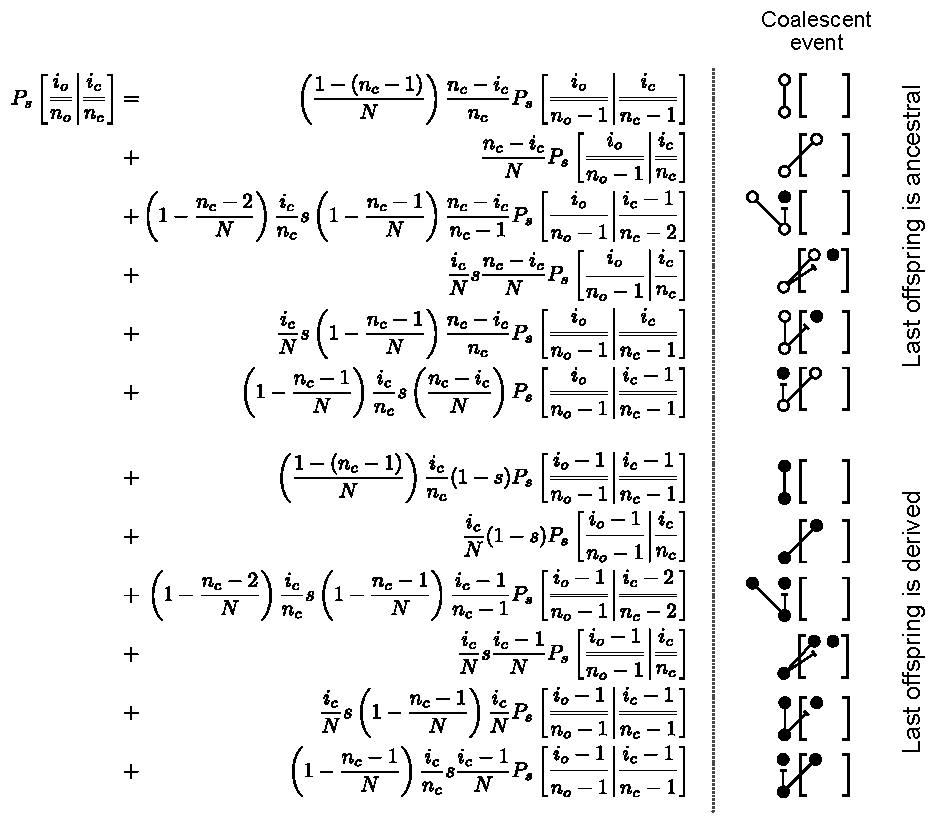
\includegraphics[width=0.9\textwidth]{fig/recurrence-selection-annotated.pdf}
  \caption{Recurrence defining transition probabilities in a model with selection \sgcomment{I think there are some problems with the way fractions are defined, e.g. the first term should start with $1-\frac{n_c-1}{N}$, not $\frac{1-(n_c-1)}{N}$ }. Right panel
    shows coalescent events corresponding to each summand. Each transition probability is defined in
    terms of transition in a smaller sample size. First six terms are conditional on the last
    offspring having an ancestral state, last six -- derived. Filled circles -- derived alleles;
    empty circles - ancestral alleles; square brackets -- smaller sample.}
  \label{fig:rec-selection}
\end{figure}

For each calculation, the ranges of the variables are:

\begin{equation}
  \begin{aligned}
    n_p &= n \\
    i_p &\in [0, n] \\
    n_c &\in [1, n] \\
    i_c &\in [0, n_c] \\
  \end{aligned}
\end{equation}

Note that unlike in the neutral case $n_c$ is now variable. The base cases of the recurrence are:

\begin{equation*}
  \begin{aligned}
    P\left[ \Dfrac{1}{1} \cond \Dfrac{1}{1} \right] &= 1-s \\
    P\left[ \Dfrac{0}{1} \cond \Dfrac{0}{1} \right] &= 1 \\
    P\left[ \Dfrac{1}{1} \cond \Dfrac{2}{2} \right] &= s \\
    P\left[ \Dfrac{0}{1} \cond \Dfrac{1}{2} \right] &= \frac{1}{s} \\
    \text{otherwise} &\phantom{{}=} 0
  \end{aligned}
\end{equation*}


\end{document}
